\documentclass[12pt,a4paper]{article}

% ─── Page Layout ───────────────────────────────────────────────────────────────
\usepackage[a4paper, margin=0.8in, headheight=14pt]{geometry}

% ─── Fonts (XeLaTeX) ───────────────────────────────────────────────────────────
\usepackage{fontspec}
\usepackage{unicode-math}
\setmainfont{TeX Gyre Pagella}
\setmonofont[Scale=0.88]{TeX Gyre Cursor}
\setmathfont{Latin Modern Math}

% ─── Packages ──────────────────────────────────────────────────────────────────
\usepackage{xcolor}
\usepackage{colortbl}
\usepackage{titlesec}
\usepackage{enumitem}
\usepackage{tabularx}
\usepackage{longtable}
\usepackage{booktabs}
\usepackage{array}
\usepackage{amsmath}
\usepackage{tikz}
\usetikzlibrary{shapes.geometric, arrows.meta, positioning, calc, fit, decorations.pathreplacing, patterns}
\usepackage{tcolorbox}
\tcbuselibrary{skins, breakable}
\usepackage{hyperref}
\usepackage{fancyhdr}
\usepackage{graphicx}
\usepackage{microtype}
\hyphenpenalty=10000
\exhyphenpenalty=10000
\sloppy
\usepackage{caption}
\usepackage{setspace}
\usepackage{multirow}
\usepackage{tocloft}

% ─── Q&A helper ────────────────────────────────────────────────────────────────
\newcommand{\Q}[1]{\textbf{#1}\par\noindent\ignorespaces}

% ─── Colour Palette ────────────────────────────────────────────────────────────
\definecolor{myred}{RGB}{196,30,58}
\definecolor{mydark}{RGB}{30,30,50}
\definecolor{mygreen}{RGB}{14,120,80}
\definecolor{myteal}{RGB}{0,130,140}
\definecolor{myamber}{RGB}{180,100,0}
\definecolor{mypurple}{RGB}{100,30,160}
\definecolor{mygray}{RGB}{246,247,249}
\definecolor{mgframe}{RGB}{180,185,200}
\definecolor{watermark}{RGB}{145,150,170}
\definecolor{hdrred}{RGB}{250,232,235}
\definecolor{hdrgreen}{RGB}{220,244,233}
\definecolor{hdrteal}{RGB}{220,242,244}
\definecolor{hdramber}{RGB}{253,242,215}
\definecolor{hdrpurple}{RGB}{238,228,255}
\definecolor{hdrgray}{RGB}{238,240,245}

% ─── Section Formatting ────────────────────────────────────────────────────────
\titleformat{\section}
  {\large\bfseries\color{myred}}{\thesection.}{0.5em}{}
  [\vspace{1pt}{\color{myred}\rule{\linewidth}{0.8pt}}]
\titleformat{\subsection}
  {\normalsize\bfseries\color{myteal}}{\thesubsection}{0.5em}{}
\titlespacing*{\section}{0pt}{18pt}{7pt}
\titlespacing*{\subsection}{0pt}{11pt}{4pt}

% ─── Paragraph ─────────────────────────────────────────────────────────────────
\setlength{\parindent}{0pt}
\setlength{\parskip}{4pt}

% ─── TOC Styling ───────────────────────────────────────────────────────────────
\renewcommand{\cfttoctitlefont}{\large\bfseries\color{myred}}
\renewcommand{\cftaftertoctitle}{\par\noindent{\color{myred}\rule{\linewidth}{0.8pt}}}
\setlength{\cftbeforetoctitleskip}{0pt}
\setlength{\cftaftertoctitleskip}{6pt}
\renewcommand{\cftsecfont}{\normalsize\bfseries\color{mydark}}
\renewcommand{\cftsecpagefont}{\normalsize\bfseries\color{mydark}}
\renewcommand{\cftsecleader}{\cftdotfill{\cftdotsep}}
\setlength{\cftbeforesecskip}{7pt}
\renewcommand{\cftsubsecfont}{\small\color{mydark}}
\renewcommand{\cftsubsecpagefont}{\small\color{mydark}}
\setlength{\cftbeforesubsecskip}{3pt}
\setlength{\cftsubsecindent}{1.4em}

% ─── Table helpers ─────────────────────────────────────────────────────────────
\renewcommand{\arraystretch}{1.45}
\setlength{\tabcolsep}{6pt}
\arrayrulecolor{mydark}
\newcolumntype{B}[1]{>{\small\bfseries\raggedright\arraybackslash}m{#1}}
\newcolumntype{Y}{>{\small\raggedright\arraybackslash}X}
\renewcommand{\tabularxcolumn}[1]{m{#1}}

% ─── Header / Footer ───────────────────────────────────────────────────────────
\pagestyle{fancy}
\fancyhf{}
\fancyhead[L]{\small\color{myred}\textbf{BS-B401}\;\color{mydark}--- Biology for Engineers}
\fancyhead[R]{\small\color{myteal}\textbf{Module 9 Notes}}
\fancyfoot[C]{\small\color{mydark}\thepage}
\fancyfoot[R]{\small\color{watermark}\textit{\copyright\ Biraj Sarkar (CGEC)}}
\renewcommand{\headrulewidth}{0.5pt}
\renewcommand{\footrulewidth}{0.3pt}

% ─── Hyperref ──────────────────────────────────────────────────────────────────
\hypersetup{
  colorlinks=true, linkcolor=myteal, urlcolor=myteal,
  pdfauthor={Biraj Sarkar (CGEC)},
  pdftitle={BS-B401 --- Module 9 Notes: Microbiology}
}

% ─── tcolorbox styles ──────────────────────────────────────────────────────────
\tcbset{
  tikzbox/.style={
    colback=mygray, colframe=mgframe, boxrule=0.6pt, arc=4pt,
    left=8pt, right=8pt, top=6pt, bottom=6pt,
    colbacktitle=mgframe, coltitle=mydark, fonttitle=\small\bfseries
  },
  defbox/.style={
    colback=hdrgreen, colframe=mygreen, boxrule=0.8pt, arc=4pt,
    left=9pt, right=9pt, top=6pt, bottom=6pt,
    colbacktitle=mygreen, coltitle=white, fonttitle=\small\bfseries
  },
  formulabox/.style={
    colback=hdrteal, colframe=myteal, boxrule=0.8pt, arc=4pt,
    left=9pt, right=9pt, top=7pt, bottom=7pt,
    colbacktitle=myteal, coltitle=white, fonttitle=\small\bfseries
  },
  examplebox/.style={
    colback=hdramber, colframe=myamber, boxrule=0.8pt, arc=4pt,
    left=9pt, right=9pt, top=6pt, bottom=6pt,
    colbacktitle=myamber, coltitle=white, fonttitle=\small\bfseries
  },
  masonbox/.style={
    colback=hdrpurple, colframe=mypurple, boxrule=0.8pt, arc=4pt,
    left=9pt, right=9pt, top=6pt, bottom=6pt,
    colbacktitle=mypurple, coltitle=white, fonttitle=\small\bfseries
  },
  exambox/.style={
    colback=hdrpurple, colframe=mypurple, boxrule=1pt, arc=5pt,
    left=10pt, right=10pt, top=8pt, bottom=8pt,
    colbacktitle=mypurple, coltitle=white, fonttitle=\bfseries,
    breakable, title after break={\textbf{Frequently Asked / Viva Questions (contd.)}}
  }
}
\tcbset{breakable}
\tcbset{after={\par\color{black}}}

% ─── TikZ styles ───────────────────────────────────────────────────────────────
\tikzset{
  block/.style={rectangle, draw=myteal, fill=hdrteal,
    text width=2.4cm, align=center, minimum height=0.95cm,
    font=\small, rounded corners=3pt, line width=0.7pt},
  redblock/.style={rectangle, draw=myred, fill=hdrred,
    text width=2.4cm, align=center, minimum height=0.95cm,
    font=\small, rounded corners=3pt, line width=0.7pt},
  amberblock/.style={rectangle, draw=myamber, fill=hdramber,
    text width=2.4cm, align=center, minimum height=0.95cm,
    font=\small, rounded corners=3pt, line width=0.7pt},
  sumjunc/.style={circle, draw=myamber, fill=hdramber,
    minimum size=0.62cm, font=\small, line width=0.8pt},
  arrow/.style={-Stealth, thick, color=mydark},
  redarrow/.style={-Stealth, thick, color=myred},
  line/.style={thick, color=mydark}
}

\begin{document}

% ─── Title Page ───────────────────────────────────────────────────────────────
\begin{center}
  {\LARGE\bfseries\color{myred} BS-B401 --- Biology for Engineers}\\[5pt]
  {\normalsize\color{mydark} Semester IV \quad$\bullet$\quad 2L:1T:0P \quad$\bullet$\quad 3 Credits}\\[3pt]
  {\normalsize\color{myteal}\textbf{Module 9 Exam Notes: Microbiology}}\\[3pt]
  {\small\color{mydark} CGEC \;$|$\; B.Tech ECE (2023--27) \;$|$\; \textit{Biraj Sarkar}}
\end{center}
\vspace{2pt}
\noindent{\color{myred}\rule{\linewidth}{1.5pt}}
\vspace{2pt}

\hypersetup{linkcolor=mydark}
\tableofcontents
\hypersetup{linkcolor=myteal}
\newpage

\section{Microbiology}
\subsection{Single-celled organisms, species and strains}
\begin{tcolorbox}[defbox, title={Microorganism}]
A microorganism is a microscopic biological entity. Here the focus is on cellular microorganisms. A single cell can sense its surroundings, acquire resources, maintain a boundary and reproduce. Many bacteria, archaea, yeasts, unicellular algae and protists carry out their life processes in one cell.
\end{tcolorbox}

\begin{itemize}[leftmargin=*, itemsep=3pt, topsep=4pt]
  \item \textbf{Prokaryotic examples.} Bacteria and archaea are distinct domains. Both lack a membrane-bound nucleus.
  \item \textbf{Eukaryotic examples.} Baker's yeast is a unicellular fungus. Some algae and protists are also unicellular.
  \item \textbf{Species.} A named biological group. For microorganisms that reproduce asexually, shared ancestry, genome relatedness and consistent traits help define groups. Interbreeding alone is not a practical species test here.
  \item \textbf{Strain.} A distinguishable lineage within a species. Strains can have different observable traits while retaining the same species name.
\end{itemize}
\subsection{Identification and classification}
\par\vspace{5pt}
\begingroup
\setlength{\extrarowheight}{1pt}
\noindent\begin{tabularx}{\linewidth}{|B{3.45cm}|Y|Y|}
\hline
\textbf{Evidence} & \textbf{What it shows} & \textbf{Why combine it with other evidence?} \\ \hline
Microscopy and morphology & Cell size, shape, arrangement or visible structures. & Different species may look similar. A single image rarely establishes species. \\ \hline
Staining or cell envelope traits & Differences in cell structures and how they retain a stain. & The grouping is informative but may be shared by many lineages. \\ \hline
Biochemical observations & Characteristic activities or products under defined observations. & Traits can vary with conditions and among strains. \\ \hline
Molecular comparison & Relatedness inferred from marker sequences or broader genomic evidence. & A conserved marker can place an organism in a broad group without resolving closely related strains. \\ \hline
\end{tabularx}\par
\endgroup
\subsection{Microscopy: magnification, contrast and resolution}
\begin{tcolorbox}[defbox, title={Resolution}]
Resolution is the ability to distinguish adjacent points as separate. Magnification is how much larger an image appears, and contrast is how strongly an object differs from its background. Increasing magnification alone does not improve resolution.
\end{tcolorbox}

\par\vspace{5pt}
\begingroup
\setlength{\extrarowheight}{1pt}
\noindent\begin{tabularx}{\linewidth}{|B{3.5cm}|Y|Y|}
\hline
\textbf{Method} & \textbf{Image information} & \textbf{Typical conceptual use} \\ \hline
Bright-field light & Light transmission and visible contrast. & Observe general cell shape or prepared stained material. \\ \hline
Phase contrast & Converts optical phase differences to intensity differences. & See low-contrast transparent cells without requiring a stain for contrast. \\ \hline
Fluorescence & Detects light emitted by fluorescent molecules. & Locate a labelled structure or naturally fluorescent feature. \\ \hline
TEM / SEM & Electrons transmitted through a thin sample (TEM) or signals from a scanned surface (SEM). & TEM reveals internal organisation. SEM primarily shows surface detail. \\ \hline
\end{tabularx}\par
\endgroup
\begin{tcolorbox}[examplebox, title={Separate magnification from resolution}]
A $10\times$ ocular and a $40\times$ objective give total magnification $400\times$. For an idealised light microscope, a common lateral-resolution estimate is $d\approx0.61\lambda/\mathrm{NA}$. At wavelength $550$ nm and numerical aperture $0.65$, $d\approx516$ nm. A smaller $d$ means finer resolvable detail.
\end{tcolorbox}

\section{Ecology, Sterility and Growth}
\subsection{Ecological roles of single-celled organisms}
\begin{itemize}[leftmargin=*, itemsep=3pt, topsep=4pt]
  \item \textbf{Primary production.} Photosynthetic unicellular algae and some bacteria fix carbon and support aquatic food webs.
  \item \textbf{Decomposition.} Microorganisms recycle material from dead organisms and return nutrients to the surroundings.
  \item \textbf{Element cycles.} Different microbial groups transform carbon, nitrogen and sulfur compounds. These transformations affect soil, water and atmospheric chemistry.
  \item \textbf{Associations.} In a mutualism both partners benefit. In commensalism one benefits with little effect on the other. In competition, organisms draw on the same limiting resource.
\end{itemize}
\subsection{Sterilization and types of media}
\begin{tcolorbox}[defbox, title={Sterilization}]
Sterilization aims to eliminate viable microorganisms, including resistant spores. Disinfection reduces or inactivates many microbes on inanimate surfaces. Antisepsis refers to antimicrobial treatment of living tissue. These are different targets of treatment.
\end{tcolorbox}

\par\vspace{5pt}
\begingroup
\setlength{\extrarowheight}{1pt}
\noindent\begin{tabularx}{\linewidth}{|B{3.45cm}|Y|Y|}
\hline
\textbf{Principle} & \textbf{What it does} & \textbf{Distinction} \\ \hline
Moist or dry heat & Inactivates cells by damaging essential structures and macromolecules. & Methods differ in how heat is transferred and how well materials tolerate it. \\ \hline
Filtration & Physically removes retained particles or cells from a stream. & Removal differs from killing. \\ \hline
Radiation or chemical treatment & Causes damage to DNA or essential molecular structures, depending on the method. & Suitability depends on penetration and material compatibility. \\ \hline
\end{tabularx}\par
\endgroup
\begin{tcolorbox}[defbox, title={Growth medium}]
A medium supplies water and chemical components that support a biological measurement or growth. In general it can provide carbon and energy sources, nitrogen, mineral ions and any required growth factors. A solid medium also contains a supporting gel such as agar. Agar is usually a support rather than the main nutrient.
\end{tcolorbox}

\begin{itemize}[leftmargin=*, itemsep=2pt]
  \item \textbf{Defined medium.} Each ingredient and quantity is known, for example specified mineral salts and a carbon compound.
  \item \textbf{Complex medium.} An extract or another ingredient has incompletely known or variable composition.
  \item \textbf{Selective medium.} Favours some groups over others, so only a subset may appear in an observation.
  \item \textbf{Differential medium.} Uses a visible reaction or indicator to distinguish groups.
\end{itemize}

A medium can be liquid or solid, and the physical form is independent of whether its composition is defined or complex. A single formulation can also be both selective and differential.
\subsection{Growth phases and growth kinetics}
\begin{tcolorbox}[tikzbox, title={Conceptual batch growth curve}]
\centering
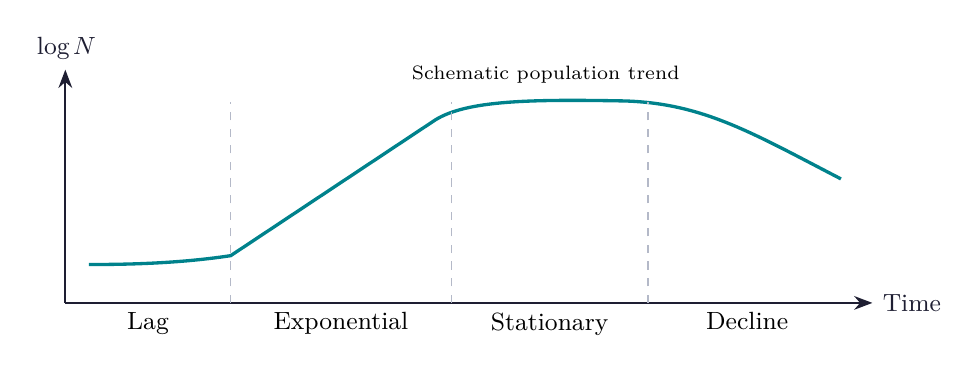
\begin{tikzpicture}[y=0.75cm,every node/.style={font=\small}]
\draw[arrow] (0,0)--(10.25,0) node[right] {Time};
\draw[arrow] (0,0)--(0,3.95) node[above,align=center] {$\log N$};
\draw[myteal,very thick] (0.3,0.65) .. controls (0.9,0.65) and (1.5,0.68) .. (2.1,0.8)
 -- (4.7,3.1) .. controls (5.1,3.43) and (5.9,3.45) .. (7.1,3.42)
 .. controls (8.1,3.38) and (8.72,2.88) .. (9.85,2.1);
\foreach \x in {2.1,4.9,7.4}{\draw[mgframe,dashed] (\x,0)--(\x,3.4);}
\node[below] at (1.05,0) {Lag};
\node[below] at (3.5,0) {Exponential};
\node[below] at (6.15,0) {Stationary};
\node[below] at (8.66,0) {Decline};
\node[font=\scriptsize,align=center] at (6.1,3.86) {Schematic population trend};
\end{tikzpicture}\par
\end{tcolorbox}

\begin{itemize}[leftmargin=*, itemsep=3pt, topsep=4pt]
  \item \textbf{Lag.} Cells adjust to changed conditions. Net population increase may be small.
  \item \textbf{Exponential.} Population increases by a nearly constant proportion per unit time. The log of count is approximately linear.
  \item \textbf{Stationary.} Total viable count levels off when net births and losses nearly balance or division slows.
  \item \textbf{Decline.} Viable count decreases. Total turbidity need not fall at the same rate as viable count.
\end{itemize}
\begin{tcolorbox}[formulabox, title={Exponential growth model}]
With constant specific growth rate $\mu$ and population $N$,
\[
\frac{dN}{dt}=\mu N,\qquad N(t)=N_0e^{\mu t},\qquad
g=\frac{\ln 2}{\mu}.
\]
For discrete doublings, $N=N_0\,2^n$ with $n=t/g$. Here $g$ is the doubling time. This model describes the exponential segment, where the assumptions approximately hold.
\end{tcolorbox}

\begin{tcolorbox}[examplebox, title={Read an illustrative population record}]
A hypothetical count increases from 100 to 800 between two measurements two hours apart. Since $800/100=2^3$, the count doubled three times. The apparent doubling time over that interval is $2/3$ hour, or 40 minutes. The specific rate is $\ln(8)/2\approx1.04\,\mathrm{h^{-1}}$. Apply this interpretation only if the interval is approximately exponential.
\end{tcolorbox}

\subsection{Interpret measurements of a microbial population}
\par\vspace{6pt}
\noindent\begin{tabularx}{\linewidth}{|B{3.4cm}|Y|Y|}
\hline
\textbf{Observation} & \textbf{What it represents} & \textbf{Interpretive limit} \\ \hline
Direct cell count & Number of visible cells in the observed sample. & Live and dead cells can both be counted unless viability is distinguished. \\ \hline
Optical density & Light scattering and attenuation by suspended material. & A proxy for total biomass or particles under comparable conditions. It can remain high after viability falls. \\ \hline
Viable count & An estimate of units capable of forming new growth in the measurement. & Clumps can behave as one unit. Some viable cells may not register in the chosen measurement. \\ \hline
\end{tabularx}\par

\begin{tcolorbox}[examplebox, title={Use an exponential-phase graph rather than one final count}]
On a graph of $\ln N$ against time, the slope in the exponential phase is $\mu$:
\[
\begin{aligned}
\ln N(t)&=\ln N_0+\mu t,\\
\mu&=\frac{\ln N_2-\ln N_1}{t_2-t_1}.
\end{aligned}
\]
This follows directly by taking the logarithm of $N(t)=N_0 e^{\mu t}$. A straight line supports a constant-rate model over that interval. Applying the same slope formula across both lag and stationary phases gives an interval average rather than the exponential growth rate.
\end{tcolorbox}

\subsection{Distinguish ecological role, identification and sterility}
\begin{itemize}[leftmargin=*, itemsep=2pt]
  \item \textbf{Ecological role.} A microscopic producer uses light or chemical energy to make organic matter from inorganic carbon. Decomposers return elements to the surroundings. Changes in one group can alter the resources available to another.
  \item \textbf{Identification.} A visible shape or staining pattern supports a broad grouping. A more specific assignment needs independent evidence. Two related strains may share a marker even if a measured trait differs.
  \item \textbf{Sterility.} A clear-looking sample is not evidence of sterility. Microscopy, turbidity and tests for viability address different questions. A physically removed cell and an inactivated cell may have the same effect on a particular count for different reasons.
\end{itemize}

\begin{tcolorbox}[masonbox, title={Answer a growth-curve question in order}]
Label the axes, explain the four phases, and identify which segment supports an exponential model. Then state whether the plotted data represent total cells, a proxy such as turbidity, or a measure of viable units. That choice determines how you explain the stationary and decline phases.
\end{tcolorbox}

\newpage
\begin{center}
  {\large\bfseries\color{myred} Quick Revision --- Module 9}\\[3pt]
  {\small\color{mydark} Microbiology $|$ BS-B401}
\end{center}
\noindent{\color{myred}\rule{\linewidth}{1.2pt}}\par\vspace{4pt}

\begin{tcolorbox}[formulabox, title={Key Concepts at a Glance}]
\renewcommand{\arraystretch}{1.35}
\noindent\begin{tabularx}{\linewidth}{B{4.5cm}Y}
Magnification & Objective magnification times ocular magnification for a simple compound microscope. \\[3pt]
Resolution & Smaller $d$ means finer detail. A common estimate is $0.61\lambda/\mathrm{NA}$. \\[3pt]
Growth & $N=N_0e^{\mu t}$ when $\mu$ is constant. $g=\ln 2/\mu$. \\[3pt]
\end{tabularx}\par
\end{tcolorbox}

\begin{tcolorbox}[defbox, title={One-Line Definitions}]
\begin{itemize}[leftmargin=*, itemsep=3pt, topsep=4pt]
  \item \textbf{Strain.} A distinguishable lineage within a species.
  \item \textbf{Sterilization.} Elimination of viable microorganisms, including resistant spores.
  \item \textbf{Defined medium.} A medium whose chemical components and amounts are specified.
\end{itemize}
\end{tcolorbox}

\begin{tcolorbox}[exambox, title={Frequently Asked / Viva Questions}]
\begin{enumerate}[topsep=0pt, label=\textbf{Q\arabic*.}, itemsep=5pt, leftmargin=*]
  \item \Q{Name a unicellular fungus used as a model.}
    Baker's yeast.
  \item \Q{Can shape alone usually identify a species?}
    Many groups share shapes, so combine independent evidence.
  \item \Q{What controls the ability to distinguish nearby points?}
    Resolution.
  \item \Q{Which method enhances contrast in transparent cells?}
    Phase contrast is one option.
  \item \Q{Name two ecological roles of microorganisms.}
    Primary production and decomposition.
  \item \Q{How do sterilization and disinfection differ?}
    Sterilization targets all viable forms. Disinfection reduces or inactivates many forms on surfaces.
  \item \Q{What does a differential medium reveal?}
    A visible reaction or other feature that distinguishes groups.
  \item \Q{What is the purpose of a solidifying agent?}
    It provides a solid support.
  \item \Q{Which growth phase gives a straight log-count graph?}
    The exponential phase under the constant-rate model.
  \item \Q{How many doublings turn 100 into 800?}
    Three, because the ratio is eight.
\end{enumerate}
\end{tcolorbox}

\begin{tcolorbox}[tikzbox, title={Summary Comparison}]
\par\vspace{5pt}
\begingroup
\setlength{\extrarowheight}{1pt}
\noindent\begin{tabularx}{\linewidth}{|B{3.45cm}|Y|Y|}
\hline
\textbf{Growth phase} & \textbf{Main observation} & \textbf{Interpretation} \\ \hline
Lag & Small change in count & Adjustment to conditions. \\ \hline
Exponential & Linear log-count trend & Approximately constant relative growth rate. \\ \hline
Stationary / decline & Plateau or fall in viable count & Net growth is near zero or negative. \\ \hline
\end{tabularx}\par
\endgroup
\end{tcolorbox}

\end{document}
